% -----------------------------------------------
% Vlastní text práce (kapitoly práce)
% -----------------------------------------------

% -----------------------------------------------
\chapter{Semiconductor detectors with p-n junction}
% -----------------------------------------------
The semiconductor structures has unique properties, which make them usable not only for a particle/photon detection. There are many types of semiconductor detectors - conventional detectors of light intensity with spectral range from infrared to UV - photoresistors and photodiodes, low intensities and single photons detectors - avalanche photodiodes (APDs), for imagining - CCD and CMOS cameras, x-ray, gamma and other particles rates and energy detectors - special photodiodes, for particle position and energy measurements - matrix drift and strip detectors. The essential role for gamma spectroscopy have the p-n junction detectors.

\par
To detect Mössbauer 14.4 keV gammas our primary choice are the Si PIN diodes for direct detection due to the high detection efficiency under 25 keV \cite{SiCdTe}. 

\section{The Structure of semiconductor}
Since we are not dealing with single atoms characterized by the well-known discrete energy levels, but with solid crystals, there is another  model describing the energy levels - the band structure. The energy levels are very close each other that they nearly form a continuum. This different behaviour is a result of a periodical potential inside the crystal lattice. However, the electron energy $E_{n}$ is not the only quantum number describing the behaviour of electrons inside the periodical potential. By solving Schrödinger equation with the help of so-called Bloch's theorem, we come to a conclusion that the second important quantum number is the wave vector $\vec{k}$. These two quantum numbers are bounded together by dispersion relations $E = E(\vec{k})$, which is characteristic for every crystal and may play role when it comes to transitions of electrons between bands.

\subsection{Band structure}
The basic difference between conductors, insulators and semiconductors is the valence and conduction band structure. In case of conductors, the valence band overlaps the conduction band. The electrons in conduction band can move nearly freely throughout the crystal. For insulators, there is no overlap, and the energy band gap $E_{\textrm{g}}$ between the two bands is so high, that it makes any transitions of electrons nearly impossible. However in case of  semiconductors, the $E_{\textrm{g}}$ is small enough to allow the electron jump into the conduction band and leaving the hole in valence band after receiving a sufficient amount of energy - in form of thermal energy $E_{\textrm{T}} = kT$, energy in static electric field $E_{\textrm{s}} = -e\phi$ or as a photon with energy quantum $E_{\textrm{photon}} = \hbar \omega$. The last one is the most important, because it allows us to use the semiconductors as detectors. Both the electron and hole participates on conduction, but they have to be treated as quasiparticles with their specific masses and mobilities.


\subsection{Occupation of states}
The occupation probability of states in band structure is given by Fermi-Dirac distribution since the electrons are the Fermions with the exclusion rules. 
\par
The possible occupied state where occupation probability drops below 50 $\%$ is called the Fermi level with Fermi energy $E_{\textrm{F}}$. 
For ideal pure semiconductor at $T=0$ K, the $E_{\textrm{F}}$ lies in the middle of the band gap. With increasing temperature, in most materials the Fermi-level moves upper towards the conduction band.

\subsection{Semiconductor Crystals}
The semiconductor materials have usually form of a crystal of diamond structure (two FCC lattices bounded together.) with the lattice atoms bounded by a covalent bond. However in real crystals there are also defects and impurities which may alter the functionality. The impurities can be added on purpose to enhance the properties we seek in procedure called doping. 
\par
The suitable materials for construction of ionizing radiation detectors are Ge - very good energy resolution, requires cooling, Si - great efficiency under 25 keV, easier fabrication since many other semiconductor devices are being made of Si and CdTe - used in wide-spectre X-Ray and Gamma Ray Detectors.
\par
The fabrication of semiconductors for purposes of detection includes many complicated processes, because the detector requirements on crystal purity are very high.

\subsection{Direct and indirect semiconductors}
 
The shape of dispersion relations $E(\vec{k})$ divides the semiconductors into two categories - direct and indirect semiconductors. For direct semiconductors the minimum in conduction band and maximum in valence band have the same $\vec{k}$, so the transition can occur after the $E_{\textrm{g}}$ is supplied. In case of indirect the minimum and maximum have different $\vec{k}$. To make transition, additional momentum has to be server (for example by phonons) or the supplied energy must be much larger to allow transition to the higher state. %with the same $\vec{k}$.  
The Si crystal is an indirect semiconductor.


 
\section{The p–n junction}
The intrinsic semiconductors have only a little field of applications. We can alter the behaviour by adding a specific impurities and create an extrinsic semiconductor. The Si atom has 4 valence electron which form a covalent bond with other Si atoms. If Si atom is replaced with atom with 5 valence electrons, one of them will have a very weak bond.
By doping the intrinsic semiconductor with these atoms we create the $n$-type with additional electrons, which are nearly localized in conduction band. However, the crystal as whole stays neutral. Similar way doping by atoms with only 3 valence electrons, there will be holes in valence band, which can participate on conduction - the $p$-type.
In band structure These atoms create energy levels in band structure, but in room temperatures, they are all mostly ionized and participate on conduction. The full theoretical treatment of doping is very complex, considers many other quantum and statistical physics aspects, and have no use for the purposes of this thesis. 

\par
The special effects will arise when $p$-type and and $n$-type are bound together. The holes from $p$-type and electrons from $n$-type will start to diffuse to the other region. However, this movement alter the charge density, which leads to creation of built-in voltage which in the end cancels the diffusion. This creates the depleted region, where are no free charge carriers. 
\par
Another theoretical view is that the electrons will rearrange, because the Fermi-level has to be same throughout the crystal, while the Fermi-level for stand-alone $p$-type is nearer to the valence band and for $n$-type is nearer to the conduction band. The potential created this way equalizes the different Fermi levels. 

\par
The p-n junction can be connected to source voltage in two ways. The $p$ layer on plus - the source voltage (refereed as bias) reduces the size of depleted layer until it completely vanishes (bias goes against built-in voltage) and the p-n junction becomes conductive - forward direction or in reverse direction - $p$ layer on minus (bias goes with built-in voltage), the size of depletion layer increases.


\par
The p-n junction has many unique properties, which are commonly used in form of classical diodes. However, it is also crucial for the detection since the free charge carriers (if somehow created) in depleted layer are pushed towards electrodes by electric field and form a photocurrent.

\par
For the purposes of design in electronic circuits, the detectors are usually modelled as classical p-n diodes, which are connected to the source of the bias voltage in reverse direction. In case of detection, the detector can be also modelled as a current source.


\par
The voltage across the depleted layer could be modelled as a simple plate capacitor. The capacitance of p-n junction plays a significant role - it alters the dynamical parameters of the detection circuits - it can alter the rising edges of pulses, alter the entire frequency spectra, increase/decrease the SNR. By varying the source voltage we vary this capacitance too.

\par
%There is also one more problem with the diffusion of electron and holes which has to be considered. It is the diffusion of charge carriers from the $p$ and $n$ layers to the metal ohmic contacts on electrodes, which can form an unwanted electric field and a potential barrier across the contact. To prevent this from happening, the regions around the ohmic contacts are highly doped to reduce the potential barrier size. 


\section{Detection mechanism}

\par
If we want to detect a particle or photon, is has to interact with the detector material - in semiconductor the creation of electron-hole pairs is observed. This could be achieved by interaction mechanisms described in previous chapters, which differ for every type of particle and energy. In case of low-energy gamma the two main mechanisms which take place in producing the charge carriers are photo-effect (internal) and Compton scattering.

\par
The main of purpose of semiconductor as a detector, is to perform a linear conversion of the particle/photon energy into the free charge carriers - electrons in conduction band and holes in valence band. The average energy needed to create a single electron-hole pair is usually a fix constant - in Si it is $\epsilon = 3.6$ eV \cite{Lutz_2007}. Since the Si is an indirect semiconductor, this value is not equal to gap energy, which is lower ($E_{\textrm{g}} = 1.12$ eV).  

\par
The gamma photon striking the detector firstly interacts with a single electron. If the photo-effect takes its place, the primary electron with energy much higher than the thermal excitation will ionize the electrons from all over the valence band pushing them into higher states from conduction band. These Electrons in conduction band de-excite themselves into lower states of conduction band and the holes redistribute themselves to the upper states in valence band. This de-excitation process releases energy again and that leads to the cascade of further excitations and interactions, which produce many electron-hole pairs - the charge cloud. Number of generated electron-hole pairs $n$ is simply given by relation:


\begin{equation}
n = \frac{E_{\textrm{gamma}}}{\epsilon}.
\end{equation}

\par
In case of Compton scattering, the scattered photon may escape the detector without any other interaction taking the rest of its energy out of the detector. This results into energy distortion. The Compton without any other interaction (Compton again or photoeffect) is typical for thin detectors since there is insufficient thickness to stop the scattered photon again. In detected gamma energy spectrum this leads into the Compton continuum with the compton edge, which devaluates the spectra.

\par
An ideal very thick detector could solve this problem, because every possible interaction and all the following sub-interactions will happen inside the detector and will result into electron-hole generation. The detector of this kind would have only the full energy peaks without any other unwanted counts. However, construction of such detector is impossible due to the many technical and manufacturing problems arising with increasing dimensions. 

\par
In case of p-n junction the created charge carriers in depleted layer are pushed towards electrodes by internal electric field. The  electronics accumulates the charge and converts it into the voltage pulse signal, which is then analysed to extract the energy information. Since the depleted layer is the only part where the detection can occur, its obvious that for detector purposes it should be large as possible. 
\par
To achieve the greater dimensions of the detection part, the p-n junction can be upgraded to p-i-n junction, which contain additional intrinsic layer between $p$ and $n$ part, which work as fix size depleted layer. The detectors with p-i-n junction are referred as PIN diodes. The additional intrinsic layer also decreases the capacitance and increases the time needed for charge carriers to exit the detection part.

\section{Main noise sources and resolution limitations}
The detection efficiency and the energy resolution are strongly dependent on noise which alters the signal. While some negative effects are caused by outer conditions such as temperature or by noise in electronics, some originate strictly from semiconductor material properties and only chance to minimize them is during the crystal's preparation.

\subsection{Fano noise}

The physical effect inside the semiconductor itself which limits the measured energy resolution is the fact that not all of the particle's energy is transformed into charge carriers. Some fraction of energy can be consumed to induce lattice vibrations (phonons). Statistically the relative resolution can be described by following equation:


\begin{equation}
\frac{\Delta E}{E} = 2.35\sqrt{\frac{F\epsilon}{E}},
\end{equation}
where $E$ is incoming particle's energy, $\epsilon$ is the average energy needed for the single pair creation and $F$ is a Fano Factor. Fano Factor is a special statistical constant which describes the dispersion in counting process. For Poisson distribution the $F$ is 1. If we consider the case of 14.4 keV gamma inside Si ($\epsilon = 3.6$ eV, $F = 0.12$), the $\frac{\Delta E}{E}$ is equal to 1.3 $\%$ and $\Delta E$ is 185.4 eV.
\par
This resolution is sometimes called intrinsic, because the real resolution is much worse. This model does not consider other sources of noise coming from the amplification in electronics, dark currents e.g. 




\subsection{Thermal noise}

It was mentioned that the electrons can be also excited by thermal fluctuations. However, since the many of detector's materials are indirect semiconductors, the thermal excitations are carried through the intermediate states inside the band gap. These states have the origin in imperfections and impurities inside the crystal lattice. The electrons and holes generated this way can join the charge cloud generated by detected particle and decrease the SNR. This phenomenon is usually called dark current.

\par
The thermal fluctuations are much more significant for materials which require less energy to excite the electrons to the conduction band such as Ge. These detectors always have to be operated at low temperatures. Even the room temperature can lead up to the breakdown and destruction of a detector. For Si, the valence and conduction band are more distant. so the thermal fluctuations are not so critical.
However, the applied bias voltage in reverse direction also increases the dark current.


\subsection{Recombination and trapping}
The effect which goes against the successful collection of charge carriers and thus affects the detection efficiency and the energy resolution is recombination. In pure crystals, the electron can recombine with hole only when they have the same $\vec{k}$. However, inside real crystals there exists impurities, which allow carriers to recombine - recombination centres. The charge collection must take much less time than it takes the carriers to recombine. 
\par
Another effect caused by the very same impurities is trapping. The trapping centres capture electron or hole and release it after certain time. This effect alter the signal pulses and can decrease maximum possible counting rate.
\par
Energy levels near the centre of band gap are primary responsible for recombination and trapping, which means that the impurities causing this are not the impurities which were added in doping, because these have their additional energy levels near the bands. 


\section{Structure and parameters of Si PIN detector}
One of the most important parameter is the size of the photosensitive area, which has to be large as possible for effective collection of radiation. This area has to be treated with extreme caution since every damage, adsorption of impurities or dew condensation due to the high environmental humidity reduces the active photosensitive area.

\par
Its obvious that for the interactions inside the detector the most crucial layer dimensions are those, which are parallel to the direction of incident radiation - the thicknesses of P and I regions.
The dead region (P) has to be thin as possible to reduce probability that the particle interacts in place where the generated charge cloud would nearly immediately recombine. The active depleted (I) layer has to be thick enough to make all the interactions happen inside itself. The schematic of PIN diode can be seen on fig. \ref{SiPIN}.


\begin{figure}[H]
 \centering
 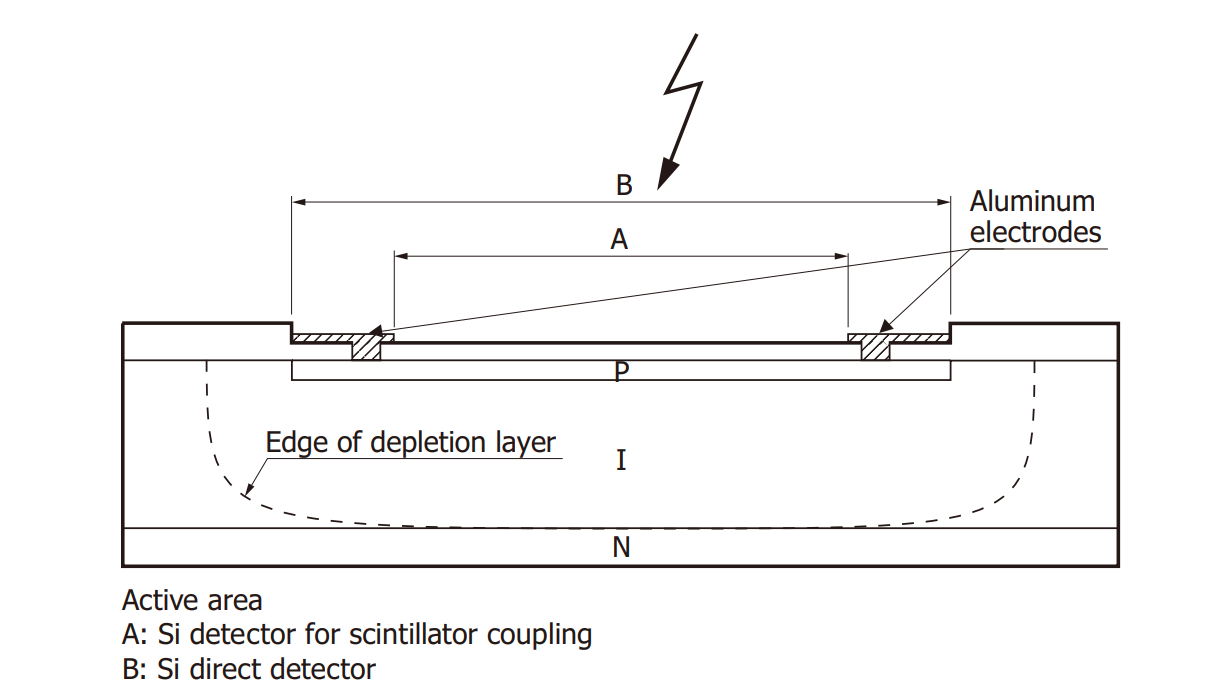
\includegraphics[scale=0.35, angle = 0]{./pictures/SiPINScheme.png}
 \caption{Cross section of Si detector for scintillator coupling and Si direct detector \cite{SiPINdirect}.}
 \label{SiPIN}
 
\end{figure}



\section{Available Si PIN detectors}
For testing we have chosen one professional Hamamatsu S14605 PIN diode and two commercial PIN diodes: OPF430 - originally designed to be used in optical fibres, BPW34 - visible and near infrared radiation detector.  

\begin{figure}[H]
 \centering
 \includegraphics[scale=0.1, angle = 0]{./pictures/PINdiodes.png}
 \caption{PIN diodes - OPF430, BPW34 and S14605.}
 \label{PIN diodes}

\end{figure}

\subsection{Hamamatsu S14605}
The professional S14605 is designed to be used as a direct radiation detector. It offers a very large photosensitive area and a low capacitance.

Parameters \cite{datS14605}:
\begin{itemize}
\item Maximum reverse voltage $U_\textrm{R}$: 150 V
\item Photosensitive area: 81 mm$^2$
\item Capacitance: 25 pF at $U_\textrm{R} = 100$ V
\item Dark current: 8 nA at $U_\textrm{R} = 100$ V
\item Depletion layer: 0.5 mm
\item Cost: 5000 CZK
\end{itemize}

%\begin{figure}[H]
% \centering
% 
\includegraphics[scale=0.35, angle = 0]{./pictures/NoPicture.jpg}
% \caption{Hamamatsu S14605.}
% \label{S14605}
% 
%\end{figure}

\subsection{OPF430}
OPF430 is originally ment to be a low-cost detector for fiber optic applications. However, there were publications \cite{RAMIREZJIMENEZ2003577}, which described the possibility of using similar diode OPF420 in low-energy gamma spectroscopic chains as a low-cost detector.

Parameters \cite{datOPF430}:
\begin{itemize}
\item Maximum reverse voltage $U_\textrm{R}$: 100 V
\item Photosensitive area: not specified, small value
\item Capacitance: 1.5  pF at $U_\textrm{R} = 5$ V
\item Dark current: 0.1 nA at $U_\textrm{R} = 5$ V
\item Depletion layer: not specified
\item Cost: 340 CZK
\end{itemize}

%\begin{figure}[H]
% \centering
% 
\includegraphics[scale=0.35, angle = 0]{./pictures/NoPicture.jpg}
% \caption{OPF430.}
% \label{OPF430}
% 
%\end{figure}

\subsection{BPW34}
BPW34 is a very low cost radiation detector. There were manuals \cite{betaBPW} how to use BPW34 as a beta particle detector, and since it is a Si PIN diode, it worths a try and test it for our gamma detection purposes.



Parameters \cite{datBPW34}:
\begin{itemize}
\item Maximum reverse voltage $U_\textrm{R}$: 32 V
\item Photosensitive area: 7.5 mm$^2$
\item Capacitance: 25 pF at $U_\textrm{R} = 3$ V
\item Dark current: 2 nA at $U_\textrm{R} = 10$ V
\item Depletion layer: not specified
\item Cost: 11 CZK
\end{itemize}

%\begin{figure}[H]
% \centering
% 
\includegraphics[scale=0.35, angle = 0]{./pictures/NoPicture.jpg}
% \caption{BPW34.}
% \label{BPW34}
% 
%\end{figure}

% %%%%%%%%%%%%%%%%%%%%%%%% End of file %%%%%%%%%%%%%%%%%%%%%%%%
